\part{附录}

\section{常用不等式}
\subsection{三角不等式}
\begin{align}
    \label{eq:三角不等式}
    \abs{x-y}     & \leq \abs{x-z} + \abs{z-y} \\
    \abs{x \pm y} & \leq \abs{x} + \abs{y}
\end{align}


\subsection{平均不等式}
从左到右为调和平均数、几何平均数、算术平均数
\begin{equation}
    \label{eq:平均不等式}
    \frac{n}{\frac{1}{x_1} + \frac{1}{x_2} + \cdots + \frac{1}{x_n}}
    \leq \sqrt[n]{x_1x_2 \cdots x_n}
    \leq \frac{x_1 + x_2 + \cdots x_n}{n}
\end{equation}
当且仅当$ x_1 = x_2 = \cdots = x_n $时,等号成立。

\subsection{面积不等式}
\begin{alignat}{1}
    \label{eq:面积不等式1} \sin x         <  x         < \tan x & \qquad (0<x<\frac{\pi}{2}) \\
    \label{eq:面积不等式2} \frac{x}{1+x}  <  \ln(1+x)  < x      & \qquad (x > -1, x \neq 0)
\end{alignat}
\begin{marginfigure}
    \centering
    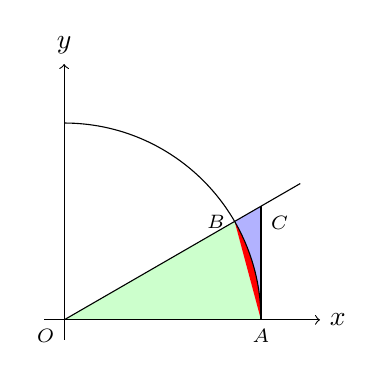
\begin{tikzpicture}[scale=2.5,domain=0:1.2]
        \coordinate[label=below left:{\scriptsize$O$}]  (O) at (0, 0);
        \coordinate[label=below:{\scriptsize$A$}]       (A) at (1, 0);
        \coordinate[label=left:{\scriptsize$B$}]        (B) at ({cos(30)}, {sin{30}});
        \coordinate[label=below right:{\scriptsize$C$}] (C) at (1, {tan(30)});

        \fill[green!20!white] (A) -- (O) -- (B) -- cycle;
        \fill[red]            (A) arc (0:30:1) -- cycle;
        \fill[blue!30!white]  (A) arc (0:30:1) -- (C) -- cycle;
        \draw (A) arc (0:90:1);
        \draw plot (\x, {tan(30)*\x});
        \draw (A) -- (C);
        \draw[->] (-0.1, 0) -- (1.3, 0) node[right] {$x$};
        \draw[->] (0, -0.1) -- (0, 1.3) node[above] {$y$};
    \end{tikzpicture}
    \caption{面积不等式\ref{eq:面积不等式1},单位圆}
    \label{fig:面积不等式1}
\end{marginfigure}
\begin{proof}
    对于不等式\ref{eq:面积不等式1},当$0<x<\frac{\pi}{2}$时,由图\ref{fig:面积不等式1}可知,$S_{\triangle AOB} < S_{\text{扇形}AOB} < S_{\triangle AOC}$,对应的值为
    \[ \frac{1}{2}\sin x < \frac{1}{2}x < \frac{1}{2}\tan x \]
\end{proof}

\begin{proof}
    对于不等式\ref{eq:面积不等式2},由\ref{fig:面积不等式2}可知,$S_{ABDC} < S_{ABDE}< S_{ABFE}$,即
    \[ \frac{x}{1+x}<\ln (1+x) < x \]
\end{proof}
\begin{marginfigure}
    \centering
    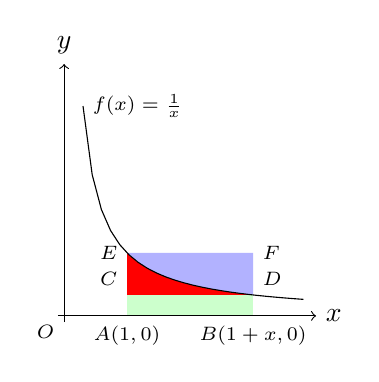
\begin{tikzpicture}[scale=0.8, declare function={f(\x)=1/\x;}]
        \coordinate[label=below left:{\scriptsize$O$}]   (O) at (0, 0);
        \coordinate[label=below:{\scriptsize$A(1,0)$}]   (A) at (1, 0);
        \coordinate[label=below:{\scriptsize$B(1+x,0)$}] (B) at (3, 0);
        \coordinate[label=above left:{\scriptsize$C$}]   (C) at (1, {f(3)});
        \coordinate[label=above right:{\scriptsize$D$}]  (D) at ({3}, {f(3)});
        \coordinate[label=left:{\scriptsize$E$}]         (E) at (1, {f(1)});
        \coordinate[label=right:{\scriptsize$F$}]        (F) at ({3}, {f(1)});

        \fill[green!20!white] (A) -- (B) -- (D) -- (C) -- cycle;
        \fill[red]            (C) -- (E) -- plot[domain=1:{3}](\x, {f(\x)}) -- cycle;
        \fill[blue!30!white]  (E) -- plot[domain=1:{3}](\x, {f(\x)}) -- (F) -- cycle;

        \draw[domain=3.8:0.3] plot (\x, {f(\x)}) node[right] {\scriptsize$f(x)=\frac{1}{x}$};
        \draw[->] (-0.1, 0) -- (4, 0)          node[right] {$x$};
        \draw[->] (0, -0.1) -- (0, 4)          node[above] {$y$};
    \end{tikzpicture}
    \caption{面积不等式\ref{eq:面积不等式2}}
    \label{fig:面积不等式2}
\end{marginfigure}

\subsection{压缩不等式}
\begin{align}
    \label{eq:压缩不等式sin} \abs{\sin x - \sin y} & \leq \abs{x - y} \\
    \label{eq:压缩不等式cos} \abs{\cos x - \cos y} & \leq \abs{x - y}
\end{align}

\subsection{阶乘不等式}
\begin{align}
    \label{eq:阶乘不等式1} 2^n < n! \leq (\frac{n+1}{2})^n & \qquad (n>4) \\
    \label{eq:阶乘不等式2} n! \geq n^{n/2}                 &
\end{align}
\begin{proof}
    不等式\ref{eq:阶乘不等式1}左侧,当$n>4$时,后续乘法$n!$总是大于$2^n$。对于右侧得不等式,根据平均不等式\ref{eq:平均不等式},
    \[ \sqrt[n]{n!} \leq \frac{1+2+\cdots+n}{n} = \frac{1+n}{2} \]
    由此可知当$n>1$时,$n! < (\frac{n+1}{2})^n$
\end{proof}
\begin{proof}
    对于不等式\ref{eq:阶乘不等式2},只需证明$\sqrt[n]{n!} \geq \sqrt{n}$,联想到平均不等式\ref{eq:平均不等式},只证明要下述不等式即可
    \[ \sqrt[n]{n!} \geq \frac{n}{1 + \frac{1}{2} + \cdots + \frac{1}{n}} \geq \sqrt{n} \]
    即
    \[ \sqrt{n} = \frac{n}{\sqrt{n}} > 1 + \frac{1}{2} + \cdots + \frac{1}{n} \]

    令$x_n=1+\frac{1}{2}+\frac{1}{3}+\cdots+\frac{1}{n}-\sqrt{n}$,则有$x_5 < 0$,并在$n>3$时有
    \begin{alignat*}{1}
        x_{n+1}-x_{n} & =    \frac{1}{n+1} + \sqrt{n} - \sqrt{n-1}  =  \frac{1}{n+1} - \frac{1}{\sqrt{n} + \sqrt{n+1}} \\
                      & \leq \frac{1}{n+1} - \frac{1}{2\sqrt{n+1}} = \frac{2 - \sqrt{n+1}}{2(n+1)} < 0
    \end{alignat*}
    所以在$n \geq 5$时,$x_n < 0$,因而有
    \[ \sqrt[n]{n!} \geq \frac{n}{1 + \frac{1}{2} + \cdots + \frac{1}{n}} > \frac{n}{\sqrt{n}} = \sqrt{n} \]
    而对于$n<5$,直接验证不等式\ref{eq:阶乘不等式2}即可。
\end{proof}

\subsection{夹挤不等式}
\begin{alignat}{2}
    \label{eq:夹挤不等式1} 2(\sqrt{n+1}-\sqrt{n}) & < \frac{1}{\sqrt{n}} & < 2(\sqrt{n}-\sqrt{n-1}) \\
    \label{eq:夹挤不等式2} \ln( 1+\frac{1}{n} )   & < \frac{1}{n}        & < \ln(1 + \frac{1}{n-1})
\end{alignat}

\subsection{柯西不等式}
\begin{align}
    \label{eq:柯西不等式}
    \left(\int_a^b f(x)g(x)\dd{x} \right)^2 & \leq \left( \int_a^bf^2(x)\dd{x} \right) \left( \int_a^bg^2(x)\dd{x} \right) & \text{积分形式}
\end{align}

\subsection{闵可夫斯基不等式}
\begin{align}
    \label{eq:闵可夫斯基不等式}
    \left( \int_a^b[f(x)+g(x)]^2\dd{x} \right)^{1/2}
    \leq
    \left( \int_a^bf^2(x)\dd{x} \right)^{1/2} +\left( \int_a^bg^2(x)\dd{x} \right)^{1/2}
\end{align}

\section{导数表}
\subsection{指数函数、对数函数}
\begin{multicols}{2}
    \begin{enumerate}
        \item $(x^\alpha)' = \alpha x^{\alpha-1}$
        \item $(a^x)' = a^x\ln a \qquad (a>0, a\neq 1)$
        \item $(\log_a x)' = \frac{1}{x\ln a} \qquad(a>0,a\neq 1)$
    \end{enumerate}
\end{multicols}

\subsection{三角函数、反三角函数}
\begin{multicols}{2}
    \begin{enumerate}
        \item $(\tan x)' =  \sec^2 x =  \frac{1}{\cos^2 x}$
        \item $(\cot x)' = -\csc^2 x = -\frac{1}{\sin^2 x}$
        \item $(\sec x)' =  \tan x\sec x$
        \item $(\csc x)' = -\cot x\csc x$
        \item $(\arcsin x)' = \frac{1}{\sqrt{1-x^2}} \qquad (\abs{x} < 1)$
        \item $(\arccos x)' =-\frac{1}{\sqrt{1-x^2}} \qquad (\abs{x} < 1)$
        \item $(\arctan x)' = \frac{1}{1+x^2}$
        \item $(\arccot x)' =-\frac{1}{1+x^2}$
    \end{enumerate}
\end{multicols}

\subsection{双曲函数、反双曲函数}
\begin{enumerate}
    \item $(\sinh x)' = \cosh x$
    \item $(\cosh x)' = \sinh x$
    \item $(\tanh x)' = \frac{1}{\cosh^2 x}$
\end{enumerate}
\begin{enumerate}[\textcolor{red}{$\bigstar$}]
    \item $(\sinh^{-1} x)' = (\ln (x+\sqrt{x^2 + 1}))' = \frac{1}{\sqrt{x^2 + 1}}$
    \item $(\cosh^{-1} x)' = (\ln (x+\sqrt{x^2 - 1}))' = \frac{1}{\sqrt{x^2 - 1}} \qquad (\abs{x} > 1)$
    \item $(\tanh^{-1} x)' = (\frac{1}{2}\ln \frac{1+x}{1-x})' = \frac{1}{1-x^2} \qquad (\abs{x} < 1)$
\end{enumerate}

\subsection{部分高阶导数}
\begin{enumerate}
    \item $(a^x)^{(n)} = a^x\ln^n a$
    \item $(\sin kx)^{(n)} = k^n \sin(kx+n\cdot \frac{\pi}{2})$ (导一次,加半$\pi$)
    \item $(\cos kx)^{(n)} = k^n \cos(kx+n\cdot \frac{\pi}{2})$ (导一次,加半$\pi$)
\end{enumerate}

\section{常用泰勒展开}
以下泰勒展开中$(x\to 0)$
\begin{enumerate}
    \item $\mathrm{e}^x = 1 + x + \dfrac{x^2}{2!} + \cdots + \dfrac{x^n}{n} + o(x^n)$
    \item $\ln(1+x) = x - \dfrac{1}{2}x^2 + \dfrac{1}{3}x^3 -\cdots+(-1)^{n+1}\dfrac{1}{n}x^n + o(x^n)$
    \item $\sin x = x-\dfrac{x^3}{3!} + \dfrac{x^5}{5!} -\cdots +(-1)^{n+1}\dfrac{x^{2n-1}}{(2n-1)!}+o(x^{2n-1})$
    \item $\cos x = 1 - \dfrac{x^2}{2!} + \dfrac{x^4}{4!} - \cdots + (-1)^n\dfrac{x^{2n}}{(2n)!} + o(x^{2n})$
    \item $\arctan x = x - \dfrac{x^3}{3} + \cdots +(-1)^{n+1}\dfrac{x^{2n-1}}{2n-1}+o(x^{2n-1})$
    \item $(1+x)^\alpha = 1 + \alpha x +\dfrac{\alpha(\alpha-1)}{2!}x^2 + \dfrac{\alpha(\alpha-1)(\alpha-2)}{3!}x^3 + o(x^3)$
    \item $\tan x = x + \dfrac{1}{3}x^3 + \dfrac{2}{15}x^5 + o(x^5)$
\end{enumerate}

\section{常微分方程解法总结}
\begin{fullpage}
    \begin{tabularx}{\textwidth}{@{}XXX@{}}
        \toprule
        \multicolumn{1}{c}{微分方程}                                                                   & \multicolumn{1}{c}{解法}                                             & \multicolumn{1}{c}{通解}                                                           \\
        \midrule
        \rowcolor{gray!40}
        \multicolumn{3}{c}{可分离方程}                                                                                                                                                                                                                             \\
        一阶,变量$x$和$y$均可分离(一般情况, 下面有特殊情况)\[P_1(x)Q_1(y)+P_2(x)Q_2(y)\dv{y}{x}=0\] & 分离变量(除以$P_2Q_1$)                                             & \[ \int^x \frac{P_1(t)}{P_2(t)}\dd{t} + \int^y\frac{Q_2(t)}{Q_1(t)}\dd{t} = C \]   \\
        \midrule
        一阶,变量$x$可分离 \[\dv{y}{x}=F(x)\]                                                         & 直接积分                                                             & \[ y=\int^x F(t)\dd{t} + C \]                                                      \\
        \midrule
        一阶自治,变量$y$可分离 \[ \dv{y}{x}=F(y) \]                                                   & 分离变量(除以$F$)                                                  & \[ x=\int^y \frac{\dd{t}}{F(t)} + C \]                                             \\
        \midrule
        一阶,变量$x$和$y$均可分离 \[ P(y)\dv{y}{x} + Q(x) = 0 \]                                      & 整个积分                                                             & \[ \int^y P(t)\dd{t} + \int^x Q(t)\dd{t} = C \]                                    \\
        \midrule
        \rowcolor{gray!40}
        \multicolumn{3}{c}{一般一阶微分方程}                                                                                                                                                                                                                       \\
        一阶,齐次 \[ \dv{y}{x} = F\left(\frac{y}{x}\right) \]                                         & 令$y=ux$,然后通过分离变量$u$和$x$求解                               & \[ \ln(Cx) = \int^{\frac{y}{x}} \frac{\dd{t}}{F(t)-t} \]                           \\
        \midrule
        一阶,可分离变量 \[ y=M(xy) + xN(xy)\dv{y}{x} = 0 \]                                           & 根据$\dd{\ln(xy)}=\frac{\dd{x}}{x} + \frac{\dd{y}}{y}$,方程除以$xy$ & \[ \ln(Cx) = \int^{xy} = \frac{N(t)\dd{t}}{t[N(t)-M(t)]} \]如果$N=M$,则解为$xy=C$ \\
        \midrule
        恰当微分,一阶 \[ M(x,y)\dv{y}{x} + N(x,y) = 0 \] 其中$\displaystyle \pdv{M}{x}=\pdv{N}{y}$    & 整个积分                                                             &
        {\[\begin{split}F(x,y) = & \int^y M(x,t)\dd{t} + \int^x N(t,y)\dd{t} \\& + Y(y) +X(x) = C\end{split}\]} 其中$Y(y)$和$X(x)$时积分处理的函数而不是常数,将他们列在这里以使最终函数$F(x,y)$满足初始条件                                                                                                                              \\
        \bottomrule
    \end{tabularx}
\end{fullpage}

\begin{fullpage}
    \begin{tabularx}{\textwidth}{@{}XXX@{}}
        \toprule
        \multicolumn{1}{c}{微分方程}                                                                   & \multicolumn{1}{c}{解法}                                                                                                                                                   & \multicolumn{1}{c}{通解}                                             \\
        \midrule
        \rowcolor{gray!40}
        \multicolumn{3}{c}{一般一阶微分方程}                                                                                                                                                                                                                                                                                                               \\
        反常微分, 一阶 \[ M(x,y)\dv{y}{x} + N(x,y) = 0 \] 其中$\displaystyle \pdv{M}{x}\neq\pdv{N}{y}$ & 积分变量$\mu(x,y)$ 满足\[\pdv{(\mu M)}{x}=\pdv{(\mu N)}{y}\]                                                                                                               & 如果可以得到$\mu(x,y)$
        {\[\begin{split}F(x,y) = & \int^y \mu(x,t)M(x,t)\dd{t} \\ &+ \int^x \mu(t,y)N(t,y)\dd{t} \\& + Y(y) +X(x) = C\end{split}\]}                                                                                                                                                                                                                                                                                                                   \\
        \midrule
        \rowcolor{gray!40}
        \multicolumn{3}{c}{一般二阶微分方程}                                                                                                                                                                                                                                                                                                               \\
        二阶, 自治\[ \dv[2]{y}{x} = F(y) \]                                                            & 原方程乘以$\displaystyle 2\dv{y}{x}$,代换$2\dv{y}{x}\dv[2]{y}{x} = \dv{x}(\dv{y}{x})^2$然后两次积分                                                                       & \[ x=\pm\int^y \frac{\dd{t}}{\sqrt{2\int^t F(m)\dd{m}} +C_1} +C_2 \] \\
        \midrule
        \rowcolor{gray!40}
        \multicolumn{3}{c}{线性方程}                                                                                                                                                                                                                                                                                                                       \\
        一阶线性,非齐次的函数系数\[ \dv{y}{x + P(x)y = Q(x)} \]                                       & 积分因子$\mathrm{e}^{\int^x P(t)\dd{t}}$                                                                                                                                   &
        \[\begin{split} y = \mathrm{e}^{-\int^x P(s)\dd{s}}\left[\int^x \mathrm{e}^{\int^t P(m)\dd{m}}Q(t)\dd{t}\right.\\ + \left.C \vphantom{\int^x}\right]\end{split} \]                                                                                                                                                                                                                                                                                                                    \\
        \midrule
        二阶线性,非齐次的常系数\[ \dv[2]{y}{x}+b\dv{y}{x} + cy = r(x) \]                              & 设$y_c=\mathrm{e}^{\alpha x}$代换并解出$\alpha$中的多项式,求出线性无关函数$\mathrm{e}^{\alpha_j x}$,特解$y_p$一般运用常数变易法, 虽然对于非常容易的$r(x)$可以直观判断。 &                                                                      \\
        \bottomrule
    \end{tabularx}
\end{fullpage}

\section{线性代数相关公式}
\subsection{伴随矩阵的公式}\label{sec:伴随矩阵的公式}

设$A$为$n$阶矩阵
\begin{enumerate}[(1)]
    \item $AA^*=A^*A=|A|E$;
    \item $(kA)^* = k^{n-1}A^*$;
    \item $(A^*)^\intercal = (A^\intercal)^*$;
    \item $|A^*|=|A|^{n-1}$;
    \item $(A^*)^*=|A|^{n-2}A$;
    \item $(A^*)^{-1} = (A^{-1})^* = \dfrac{1}{|A|}A$;
    \item $
              r(A^*) =
              \begin{cases}
                  n, & r(A)=n,   \\
                  1, & r(A)=n-1, \\
                  0, & r(A)<n-1.
              \end{cases}
          $
\end{enumerate}

\subsection{矩阵的秩相关公式}
\label{sec:矩阵的秩相关公式}

\begin{enumerate}[(1)]
    \item $r(A^\intercal) = r(A)$;
    \item $r(kA) = r(A), k\neq 0$;
    \item $r(0E - A) = r(A)$;
    \item $r(A-E) = r(E-A)$;
    \item $r(A+B)\leq r(A) + r(B)$;
    \item $r(AB)\leq \min(r(A),r(B))$;
    \item 若$A$可逆,则$r(AB)=r(BA)=r(B)$;
    \item $r(A^\intercal A) = r(A )$;
    \item 西尔维斯特不等式\label{eq:西尔维斯特不等式}:$A_{m\times n}, B_{n\times s}$,则$r(A)+r(B)-n\leq r(AB)$;
    \item $
              r\begin{pmatrix}
                  A & 0 \\
                  0 & B
              \end{pmatrix}
              =r(A)+r(B)
          $
    \item $A\sim B$,则$r(A)=r(B), r(A+kE)=r(B+kE)$
\end{enumerate}

\subsection{可逆矩阵的性质}\label{sec:可逆矩阵的性质}
设矩阵$A,B$可逆,$k=\neq 0$,则有如下性质
\begin{enumerate}[(1)]
    \item $A^{-1}$可逆,$(A^{-1})^{-1} = A$;
    \item $kA$可逆,$(kA^{-1}) = \frac{1}{k} A^{-1}$;
    \item $AB$可逆,$(AB)^{-1} = A^{-1}B^{-1}$;
    \item $A^\intercal$可逆,$(A^\intercal)^{-1} = (A^{-1})^\intercal$。
\end{enumerate}